%%%%%%%%%%%%%%%%%%%%%%%%%%%%%%%%%%%%%%%%%
% Masters/Doctoral Thesis 
% LaTeX Template
% Version 2.5 (27/8/17)
%
% This template was downloaded from:
% http://www.LaTeXTemplates.com
%
% Version 2.x major modifications by:
% Vel (vel@latextemplates.com)
%
% This template is based on a template by:
% Steve Gunn (http://users.ecs.soton.ac.uk/srg/softwaretools/document/templates/)
% Sunil Patel (http://www.sunilpatel.co.uk/thesis-template/)
%
% Template license:
% CC BY-NC-SA 3.0 (http://creativecommons.org/licenses/by-nc-sa/3.0/)
%
%%%%%%%%%%%%%%%%%%%%%%%%%%%%%%%%%%%%%%%%%

%----------------------------------------------------------------------------------------
%	PACKAGES AND OTHER DOCUMENT CONFIGURATIONS
%----------------------------------------------------------------------------------------

\documentclass[
11pt, % The default document font size, options: 10pt, 11pt, 12pt
oneside, % Two side (alternating margins) for binding by default, uncomment to switch to one side
spanish, % ngerman for German
singlespacing, % Single line spacing, alternatives: onehalfspacing or doublespacing
%draft, % Uncomment to enable draft mode (no pictures, no links, overfull hboxes indicated)
%nolistspacing, % If the document is onehalfspacing or doublespacing, uncomment this to set spacing in lists to single
%liststotoc, % Uncomment to add the list of figures/tables/etc to the table of contents
%toctotoc, % Uncomment to add the main table of contents to the table of contents
% parskip, % Uncomment to add space between paragraphs
%nohyperref, % Uncomment to not load the hyperref package
headsepline, % Uncomment to get a line under the header
%chapterinoneline, % Uncomment to place the chapter title next to the number on one line
%consistentlayout, % Uncomment to change the layout of the declaration, abstract and acknowledgements pages to match the default layout
]{MastersDoctoralThesis} % The class file specifying the document structure

\usepackage[utf8]{inputenc} % Required for inputting international characters
\usepackage[T1]{fontenc} % Output font encoding for international characters

\usepackage{mathpazo} % Use the Palatino font by default
\usepackage{lipsum}
\usepackage[acronym, toc]{glossaries}
\usepackage{amsmath}
\usepackage{amssymb}
\usepackage{float}
\usepackage{todonotes}
\usepackage{bm}
\usepackage{subfigure}
\usepackage{amsfonts}
\usepackage{amsthm}
\usepackage{multirow}
\usepackage{colortbl}
% \usepackage{booktabs}
% \usepackage{makeidx}\makeindex

\usepackage[backend=bibtex,style=numeric,natbib=true]{biblatex} % Use the bibtex backend with the authoryear citation style (which resembles APA)

\addbibresource{references.bib} % The filename of the bibliography

\usepackage[autostyle=true]{csquotes} % Required to generate language-dependent quotes in the bibliography

% \usepackage[letterpaper,landscape,margin=3cm]{geometry}
\usepackage{tikz}
\usetikzlibrary{calc}

% GanttHeader setups some parameters for the rest of the diagram
% #1 Width of the diagram
% #2 Width of the space reserved for task numbers
% #3 Width of the space reserved for task names
% #4 Number of months in the diagram
% In addition to these parameters, the layout of the diagram is influenced
% by keys defined below, such as y, which changes the vertical scale
\def\GanttHeader#1#2#3#4{%
 \pgfmathparse{(#1-#2-#3)/#4}
 \tikzset{y=7mm, task number/.style={left, font=\bfseries},
     task description/.style={text width=#3,  right, draw=none,
           font=\sffamily, xshift=#2,
           minimum height=2em},
     gantt bar/.style={draw=black, fill=red!50!black},
     help lines/.style={draw=black!30, dashed},
     x=\pgfmathresult pt
     }
  \def\totalmonths{#4}
  \node (Header) [task description] at (0,0) {\textbf{\large Actividades}};
  \begin{scope}[shift=($(Header.south east)$)]
    \foreach \x in {1,...,#4}
      \node[above] at (\x,0) {\footnotesize\x};
 \end{scope}
}

% This macro adds a task to the diagram
% #1 Number of the task
% #2 Task's name
% #3 Starting date of the task (month's number, can be non-integer)
% #4 Task's duration in months (can be non-integer)
\def\Task#1#2#3#4{%
\node[task number] at ($(Header.west) + (0, -#1)$) {#1};
\node[task description] at (0,-#1) {#2};
\begin{scope}[shift=($(Header.south east)$)]
  \draw (0,-#1) rectangle +(\totalmonths, 1);
  \foreach \x in {1,...,\totalmonths}
    \draw[help lines] (\x,-#1) -- +(0,1);
  \filldraw[gantt bar] ($(#3, -#1+0.2)$) rectangle +(#4,0.6);
\end{scope}
}

%----------------------------------------------------------------------------------------
%	MARGIN SETTINGS
%----------------------------------------------------------------------------------------

\geometry{
	paper=letterpaper, % Change to letterpaper for US letter
	inner=2.5cm, % Inner margin
	outer=3.8cm, % Outer margin
	bindingoffset=.5cm, % Binding offset
	top=1.5cm, % Top margin
	bottom=1.5cm, % Bottom margin
	%showframe, % Uncomment to show how the type block is set on the page
}

%----------------------------------------------------------------------------------------
%	THESIS INFORMATION
%----------------------------------------------------------------------------------------

\thesistitle{Advanced Natural Language Processing Techniques to Profile Cybercriminals} % Your thesis title, this is used in the title and abstract, print it elsewhere with \ttitle
\supervisor{Dr. Daniel Orlando \textsc{D\'{\i}az L\'opez}} % Your supervisor's name, this is used in the title page, print it elsewhere with \supname
\examiner{} % Your examiner's name, this is not currently used anywhere in the template, print it elsewhere with \examname
\degree{Estudiante de Ingeniería de Sistemas} % Your degree name, this is used in the title page and abstract, print it elsewhere with \degreename
\author{Alejandro \textsc{Anzola \'Avila}} % Your name, this is used in the title page and abstract, print it elsewhere with \authorname
\addresses{} % Your address, this is not currently used anywhere in the template, print it elsewhere with \addressname

\subject{Computer Science} % Your subject area, this is not currently used anywhere in the template, print it elsewhere with \subjectname
\keywords{Natural Language Processing, NLP, Cybercriminal} % Keywords for your thesis, this is not currently used anywhere in the template, print it elsewhere with \keywordnames
\university{\href{https://www.escuelaing.edu.co}{Escuela Colombiana de Ingeniería\\Julio Garavito}} % Your university's name and URL, this is used in the title page and abstract, print it elsewhere with \univname
\department{\href{https://www.escuelaing.edu.co/es/programas/pregrado/Ingenier\%C3\%ADa+de+Sistemas}{Programa de Ingeniería de Sistemas}} % Your department's name and URL, this is used in the title page and abstract, print it elsewhere with \deptname
\group{\href{ }{ }} % Your research group's name and URL, this is used in the title page, print it elsewhere with \groupname
% \faculty{\href{http://faculty.university.com}{Faculty Name}} % Your faculty's name and URL, this is used in the title page and abstract, print it elsewhere with \facname
\faculty{} % Your faculty's name and URL, this is used in the title page and abstract, print it elsewhere with \facname

\AtBeginDocument{
\hypersetup{linkcolor=red!50!black} % set links colors (added myself)
\hypersetup{pdftitle=\ttitle} % Set the PDF's title to your title
\hypersetup{pdfauthor=\authorname} % Set the PDF's author to your name
\hypersetup{pdfkeywords=\keywordnames} % Set the PDF's keywords to your keywords
}

\makeglossaries
% Reference: https://www.overleaf.com/learn/latex/Glossaries

\newcommand{\glossarydef}[4]{ % label, name, long, description
    \newglossaryentry{{#1}-g}{
        name={#3},
        description={{\rm #4}}
    }

%%% define the acronym and use the see= option
    \newglossaryentry{#1}{
        type=\acronymtype,
        name={#2},
        description={{\rm #3}},
        first={#3 (#2)\glsadd{{#1}-g}},
        long={#3}
        % see=[Glosario:]{{#1}g}
    }
}

\glossarydef{nlp}{NLP}{Natural Language Processing}{Rama de la inteligencia artificial que lidia con la interaccion entre computadores y humanos usando el lenguaje natural}

\glossarydef{machinel}{ML}{Machine Learning}{Informalmente ha sido definido como ``El campo de estudio que le da a computadores la habilidad de aprender sin ser explicitamente programados'', este tiene tres tipos de algortimos de aprendizaje: apredizaje supervizado, aprendizaje no--supervizado, y aprendizaje por refuerzo}

\glossarydef{deepl}{DL}{Deep Learning}{Es un subcampo de Machine Learning que se usa algorimos inspirados por la estructura y funcion del cerebro que son llamadas Redes Neuronales Artificiales (\'o Artificial Neural Networks en ingl\'es)}

\glossarydef{dataintegration}{DI}{Data Integration}{Para acceder a múltiples y diversas fuentes de información}

\glossarydef{linkanalisys}{LA}{Link Analysis}{Para visualizar asociaciones y relaciones criminales y terroristas}

\glossarydef{softwareagents}{SA}{Software Agents}{Para el monitoreo, obtención, análisis y actuación sobre la información}

\glossarydef{textmining}{TM}{Text Mining}{Búsqueda sobre terabytes de información en documentos, paginas web y correos electrónicos}

\glossarydef{neuralnetworks}{NN}{Neural Networks}{Para predecir la probabilidad de crímenes y nuevos ataques terroristas}

\glossarydef{mlalgorithms}{MLA}{Machine Learning Algoritms}{Para extraer perfiles de perpetradores y mapas gráficos de crímenes}

\glossarydef{kbs}{KBS}{Knowledge Based Systems}{{\bf Pendiente}}

\glossarydef{ai}{AI}{Artificial Intelligence}{{\bf Pendiente}}

\glossarydef{anomalydetectionsys}{ADS}{Anomaly Detection Systems}{{\bf Pendiente}}

\glossarydef{som}{SOM}{Self-organizing Maps}{{\bf Pendiente}}


\begin{document}

\frontmatter % Use roman page numbering style (i, ii, iii, iv...) for the pre-content pages

\pagestyle{plain} % Default to the plain heading style until the thesis style is called for the body content

%----------------------------------------------------------------------------------------
%	TITLE PAGE
%----------------------------------------------------------------------------------------

\begin{titlepage}
\begin{center}

\vspace*{.06\textheight}
{\scshape\LARGE \univname\par}\vspace{1.5cm} % University name
\textsc{\Large Proyecto de Grado}\\[0.5cm] % Thesis type

\HRule \\[0.4cm] % Horizontal line
{\huge \bfseries \ttitle\par}\vspace{0.4cm} % Thesis title
\HRule \\[1.5cm] % Horizontal line
 
\begin{minipage}[t]{0.4\textwidth}
\begin{flushleft} \large
\emph{Autor:}\\
\href{https://www.linkedin.com/in/alejandro-anzola-avila/}{\authorname} % Author name - remove the \href bracket to remove the link
\end{flushleft}
\end{minipage}
\begin{minipage}[t]{0.45\textwidth}
\begin{flushright} \large
\emph{Director:} \\
\href{https://dodiazlopez.github.io/main/}{\supname} % Supervisor name - remove the \href bracket to remove the link  
\end{flushright}
\end{minipage}\\[3cm]
 
\vfill

% \large \textit{A thesis submitted in fulfillment of the requirements\\ for the degree of \degreename}\\[0.3cm] % University requirement text
% \textit{in the}\\[0.4cm]
\groupname\\\deptname\\[0.5cm] % Research group name and department name
\textsc{Bogot\'a, Colombia}\\[1cm]
 
\vfill

\includegraphics[scale=0.4]{University/escuela-logo.png}\\ % University/department logo - uncomment to place it
{\large \textrm{\today}}\\%[4cm] % Date
 
\vfill
\end{center}
\end{titlepage}

%----------------------------------------------------------------------------------------
%	DECLARATION PAGE
%----------------------------------------------------------------------------------------

% \begin{declaration}
% \addchaptertocentry{\authorshipname} % Add the declaration to the table of contents
% \noindent I, \authorname, declare that this thesis titled, \enquote{\ttitle} and the work presented in it are my own. I confirm that:

% \begin{itemize} 
% \item This work was done wholly or mainly while in candidature for a research degree at this University.
% \item Where any part of this thesis has previously been submitted for a degree or any other qualification at this University or any other institution, this has been clearly stated.
% \item Where I have consulted the published work of others, this is always clearly attributed.
% \item Where I have quoted from the work of others, the source is always given. With the exception of such quotations, this thesis is entirely my own work.
% \item I have acknowledged all main sources of help.
% \item Where the thesis is based on work done by myself jointly with others, I have made clear exactly what was done by others and what I have contributed myself.\\
% \end{itemize}
 
% \noindent Signed:\\
% \rule[0.5em]{25em}{0.5pt} % This prints a line for the signature
 
% \noindent Date:\\
% \rule[0.5em]{25em}{0.5pt} % This prints a line to write the date
% \end{declaration}

% \cleardoublepage

%----------------------------------------------------------------------------------------
%	QUOTATION PAGE
%----------------------------------------------------------------------------------------

% \vspace*{0.2\textheight}

% \noindent\enquote{\itshape Thanks to my solid academic training, today I can write hundreds of words on virtually any topic without possessing a shred of information, which is how I got a good job in journalism.}\bigbreak

% \hfill Dave Barry

%----------------------------------------------------------------------------------------
%	ACKNOWLEDGEMENTS
%----------------------------------------------------------------------------------------

% \begin{acknowledgements}
% \addchaptertocentry{\acknowledgementname} % Add the acknowledgements to the table of contents
% The acknowledgments and the people to thank go here, don't forget to include your project advisor\ldots
% \end{acknowledgements}

%----------------------------------------------------------------------------------------
%	LIST OF CONTENTS/FIGURES/TABLES PAGES
%----------------------------------------------------------------------------------------

\tableofcontents % Prints the main table of contents

\listoffigures % Prints the list of figures

\listoftables % Prints the list of tables

%----------------------------------------------------------------------------------------
%	ABSTRACT PAGE
%----------------------------------------------------------------------------------------

\begin{abstract}
\addchaptertocentry{\abstractname} % Add the abstract to the table of contents
  In document language ... \todo{Escribir abstract}
\end{abstract}

\begin{extraAbstract}
In english.... \todo{Escribir abstract en ingles}
\end{extraAbstract}

%----------------------------------------------------------------------------------------
%	ABBREVIATIONS
%----------------------------------------------------------------------------------------

% \begin{abbreviations}{ll} % Include a list of abbreviations (a table of two columns)

% \textbf{LAH} & \textbf{L}ist \textbf{A}bbreviations \textbf{H}ere\\
% \textbf{WSF} & \textbf{W}hat (it) \textbf{S}tands \textbf{F}or\\

% \end{abbreviations}

%----------------------------------------------------------------------------------------
%	PHYSICAL CONSTANTS/OTHER DEFINITIONS
%----------------------------------------------------------------------------------------

% \begin{constants}{lr@{${}={}$}l} % The list of physical constants is a three column table

% % The \SI{}{} command is provided by the siunitx package, see its documentation for instructions on how to use it

% Speed of Light & $c_{0}$ & \SI{2.99792458e8}{\meter\per\second} (exact)\\
% %Constant Name & $Symbol$ & $Constant Value$ with units\\

% \end{constants}

%----------------------------------------------------------------------------------------
%	SYMBOLS
%----------------------------------------------------------------------------------------

% \begin{symbols}{lll} % Include a list of Symbols (a three column table)

% $a$ & distance & \si{\meter} \\
% $P$ & power & \si{\watt} (\si{\joule\per\second}) \\
% %Symbol & Name & Unit \\

% \addlinespace % Gap to separate the Roman symbols from the Greek

% $\omega$ & angular frequency & \si{\radian} \\

% \end{symbols}

%----------------------------------------------------------------------------------------
%	DEDICATION
%----------------------------------------------------------------------------------------

% \dedicatory{For/Dedicated to/To my\ldots} 

%----------------------------------------------------------------------------------------
%	THESIS CONTENT - CHAPTERS
%----------------------------------------------------------------------------------------

\mainmatter % Begin numeric (1,2,3...) page numbering

\pagestyle{thesis} % Return the page headers back to the "thesis" style

% Include the chapters of the thesis as separate files from the Chapters folder
% Uncomment the lines as you write the chapters

%----------------------------------------------------------------------------------------

% Define some commands to keep the formatting separated from the conten

\newcommand{\figureref}[1]{\mbox{Figura~\ref{#1}}}
\newcommand{\tableref}[1]{\mbox{Cuadro~\ref{#1}}}
\newcommand{\equationref}[1]{\mbox{Ecuación~\ref{#1}}}
\newcommand{\sectionref}[1]{\mbox{Sección~\ref{#1}}}

\newcommand{\norm}[1]{\left\lVert#1\right\rVert}
\newcommand{\keyword}[1]{\textbf{#1}}
\newcommand{\tabhead}[1]{\textbf{#1}}
\newcommand{\code}[1]{\texttt{#1}}
\newcommand{\file}[1]{\texttt{\bfseries#1}}
\newcommand{\option}[1]{\texttt{\itshape#1}}

\newlength{\figwidth}
\setlength{\figwidth}{26pc}
\newlength{\notationgap}
\setlength{\notationgap}{1pc}

% ----------------------------------------------------------------------------------------

\input{math_commands.tex} % para definir una notacion
\chapter*{Notación}
\label{notation}


% Sometimes we have to include the following line to get this section
% included in the Table of Contents despite being a chapter*
\addcontentsline{toc}{chapter}{Notación}

\vspace{\notationgap}
% Need to use minipage to keep title of table on same page as table
{\begin{center} \large Esta notación es una adaptación de la presentada en \cite{deeplearning}.\end{center}}

\begin{minipage}{\textwidth}
% This is a hack to put a little title over the table
% We cannot use "\section*", etc., they appear in the table of contents.
% tocdepth does not work on this chapter.
  
\centerline{\bf Números y Arreglos}
\bgroup
% The \arraystretch definition here increases the space between rows in the table,
% so that \displaystyle math has more vertical space.
\def\arraystretch{1.5}
\begin{tabular}{cp{0.7\textwidth}}
$\displaystyle a$ & Un escalar (entero o real)\\
$\displaystyle \va$ & Un vector\\
$\displaystyle \mA$ & Una matriz\\
% $\displaystyle \tA$ & A tensor\\
$\displaystyle \mI_n$ & Matriz identidad con $n$ filas y $n$ columnas\\
$\displaystyle \mI$ & Matriz identidad con dimensionalidad implícita por el contexto\\
$\displaystyle \ve^{(i)}$ & Vector estándar base $[0,\dots,0,1,0,\dots,0]$ con un 1 en la posición $i$\\
% $\displaystyle \text{diag}(\va)$ & A square, diagonal matrix with diagonal entries given by $\va$\\
$\displaystyle \ra$ & Una variable aleatoria real\\
$\displaystyle \rva$ & Un vector de variables aleatorias\\
$\displaystyle \rmA$ & Una matriz de variables aleatorias\\
\end{tabular}
\egroup
\index{Scalar}
\index{Vector}
\index{Matrix}
\index{Tensor}
\end{minipage}

\vspace{\notationgap}
\begin{minipage}{\textwidth}
\centerline{\bf Conjuntos y Grafos}
\bgroup
\def\arraystretch{1.5}
\begin{tabular}{cp{0.7\textwidth}}
$\displaystyle \sA$ & Un conjunto\\
$\displaystyle \R$ & El conjunto de números reales \\
$\displaystyle \Nat$ & El conjunto de números naturales \\
% NOTE: do not use \R^+, because it is ambiguous whether:
% - It includes 0
% - It includes only real numbers, or also infinity.
% We usually do not include infinity, so we may explicitly write
% [0, \infty) to include 0
% (0, \infty) to not include 0
$\displaystyle \{0, 1\}$ & El conjunto que contiene al 0 y el 1 \\
$\displaystyle \{0, 1, \dots, n \}$ & El conjunto que contiene todos lo números entre $0$ y $n$\\
$\displaystyle [a, b]$ & El intervalo real que incluye $a$ y $b$\\
$\displaystyle (a, b]$ & El intervalo real que no incluye $a$ pero si $b$ \\
$\displaystyle \sA \backslash \sB$ & Substracción de conjuntos, e.g., el conjunto que contiene los elementos de  $\sA$ que no están en $\sB$\\
$\displaystyle \gG$ & Un grafo\\
$\displaystyle \parents_\gG(\ervx_i)$ & El padre de $\ervx_i$ en $\gG$
\end{tabular}
\egroup
\index{Scalar}
\index{Vector}
\index{Matrix}
\index{Tensor}
\index{Graph}
\index{Set}
\end{minipage}

\vspace{\notationgap}
\begin{minipage}{\textwidth}
\centerline{\bf Índices}
\bgroup
\def\arraystretch{1.5}
\begin{tabular}{cp{0.7\textwidth}}
$\displaystyle \eva_i$ & Elemento $i$ del vector $\va$, con índice empezando en 1\\
$\displaystyle \eva_{-i}$ & Todos los elementos del vector $\va$ a excepción del elemento $i$ \\
$\displaystyle \emA_{i,j}$ & Elemento $i, j$ de la matriz $\mA$ \\
$\displaystyle \mA_{i, :}$ & Fila $i$ de la matriz $\mA$ \\
$\displaystyle \mA_{:, i}$ & Columna $i$ de la matriz $\mA$ \\
% $\displaystyle \etA_{i, j, k}$ & Element $(i, j, k)$ of a 3-D tensor $\tA$\\
% $\displaystyle \tA_{:, :, i}$ & 2-D slice of a 3-D tensor\\
$\displaystyle \erva_i$ & Elemento $i$ del vector aleatorio $\rva$ \\
\end{tabular}
\egroup
\end{minipage}

\vspace{\notationgap}
\begin{minipage}{\textwidth}
\centerline{\bf Operaciones de Álgebra Lineal}
\bgroup
\def\arraystretch{1.5}
\begin{tabular}{cp{0.7\textwidth}}
$\displaystyle \mA^\top$ & Traspuesta de la matriz $\mA$ \\
% $\displaystyle \mA^+$ & Moore-Penrose pseudoinverse of $\mA$\\
% $\displaystyle \mA \odot \mB $ & Element-wise (Hadamard) product of $\mA$ and $\mB$ \\
% Wikipedia uses \circ for element-wise multiplication but this could be confused with function composition
$\displaystyle \mathrm{det}(\mA)$ & Determinante de la matriz $\mA$ \\
\end{tabular}
\egroup
\index{Transpose}
\index{Element-wise product|see {Hadamard product}}
\index{Hadamard product}
\index{Determinant}
\end{minipage}

\vspace{\notationgap}
\begin{minipage}{\textwidth}
\centerline{\bf Calculo}
\bgroup
\def\arraystretch{1.5}
\begin{tabular}{cp{0.7\textwidth}}
% NOTE: the [2ex] on the next line adds extra height to that row of the table.
% Without that command, the fraction on the first line is too tall and collides
% with the fraction on the second line.
$\displaystyle\frac{d y} {d x}$ & Derivada de $y$ con respecto a  $x$\\ [2ex]
$\displaystyle \frac{\partial y} {\partial x} $ & Derivada parcial de $y$ con respecto a $x$ \\
$\displaystyle \nabla_\vx y $ & Gradiente de $y$ con respecto a $\vx$ \\
$\displaystyle \nabla_\mX y $ & Matriz de derivadas de $y$ con respecto a $\mX$ \\
% $\displaystyle \nabla_\tX y $ & Tensor containing derivatives of $y$ with respect to $\tX$ \\
% $\displaystyle \frac{\partial f}{\partial \vx} $ & Jacobian matrix $\mJ \in \R^{m\times n}$ of $f: \R^n \rightarrow \R^m$\\
% $\displaystyle \nabla_\vx^2 f(\vx)\text{ or }\mH( f)(\vx)$ & The Hessian matrix of $f$ at input point $\vx$\\
$\displaystyle \int f(\vx) d\vx $ & Integral definida sobre un dominio entero $\vx$ \\
$\displaystyle \int_\sS f(\vx) d\vx$ & Integral definida con respecto a $\vx$ sobre el conjunto $\sS$ \\
\end{tabular}
\egroup
\index{Derivative}
\index{Integral}
\index{Jacobian matrix}
\index{Hessian matrix}
\end{minipage}

\vspace{\notationgap}
\begin{minipage}{\textwidth}
\centerline{\bf Teoría de Probabilidad e Información}
\bgroup
\def\arraystretch{1.5}
\begin{tabular}{cp{0.7\textwidth}}
$\displaystyle \ra \bot \rb$ & Las variables aleatorias $\ra$ y $\rb$ son independientes\\
$\displaystyle \ra \bot \rb \mid \rc $ & Son condicionalmente independientes dado $\rc$\\
$\displaystyle P(\ra)$ & Una distribución de probabilidad de una variable aleatoria discreta\\
$\displaystyle p(\ra)$ & Una distribución de probabilidad de una variable aleatoria continua\\
$\displaystyle \ra \sim P$ & La variable aleatoria $\ra$ tiene distribución $P$\\% so thing on left of \sim should always be a random variable, with name beginning with \r
% $\displaystyle  \E_{\rx\sim P} [ f(x) ]\text{ or } \E f(x)$ & Expectation of $f(x)$ with respect to $P(\rx)$ \\
% $\displaystyle \Var(f(x)) $ &  Variance of $f(x)$ under $P(\rx)$ \\
% $\displaystyle \Cov(f(x),g(x)) $ & Covariance of $f(x)$ and $g(x)$ under $P(\rx)$\\
% $\displaystyle H(\rx) $ & Shannon entropy of the random variable $\rx$\\
% $\displaystyle \KL ( P \Vert Q ) $ & Kullback-Leibler divergence of P and Q \\
$\displaystyle \mathcal{N} ( \vx ; \vmu , \vsigma^2)$ & Distribución gaussiana %
sobre $\vx$ con media $\vmu$ y varianza $\vsigma^2$ \\
\end{tabular}
\egroup
\index{Independence}
\index{Conditional independence}
\index{Variance}
\index{Covariance}
\index{Kullback-Leibler divergence}
\index{Shannon entropy}
\end{minipage}

\vspace{\notationgap}
\begin{minipage}{\textwidth}
\centerline{\bf Funciones}
\bgroup
\def\arraystretch{1.5}
\begin{tabular}{cp{0.7\textwidth}}
$\displaystyle f: \sA \rightarrow \sB$ & La función $f$ con dominio $\sA$ y rango $\sB$\\
$\displaystyle f \circ g $ & Composición de las funciones $f$ y $g$ \\
  $\displaystyle f(\vx ; \vtheta) $ & Una función de $\vx$ parametrizado por $\vtheta$. \\
$\displaystyle \log x$ & Logaritmo natural de $x$ \\
$\displaystyle \sigma(x)$ & Función sigmoid logística, $\displaystyle \frac{1} {1 + \exp(-x)}$ \\
% $\displaystyle \zeta(x)$ & Softplus, $\log(1 + \exp(x))$ \\
$\displaystyle \| \vx \|_p $ & Norma $\normlp$ de $\vx$ \\
$\displaystyle \| \vx \| $ & Norma $\normltwo$ de $\vx$ \\
$\displaystyle x^+$ & Parte positiva de $x$, e.g., $\max(0,x)$\\
$\displaystyle \1_\mathrm{condition}$ & Es 1 si \texttt{condition} es verdadero, 0 de lo contrario\\
\end{tabular}
\egroup
\index{Sigmoid}
\index{Softplus}
\index{Norm}
\end{minipage}

% Sometimes we use a function $f$ whose argument is a scalar but apply
% it to a vector, matrix, or tensor: $f(\vx)$, $f(\mX)$, or $f(\tX)$.
% This denotes the application of $f$ to the
% array element-wise. For example, if $\tC = \sigma(\tX)$, then $\etC_{i,j,k} = \sigma(\etX_{i,j,k})$
% for all valid values of $i$, $j$ and $k$.


\vspace{\notationgap}
\begin{minipage}{\textwidth}
\centerline{\bf Datasets}
\bgroup
\def\arraystretch{1.5}
\begin{tabular}{cp{0.7\textwidth}}
% $\displaystyle \pdata$ & The data generating distribution\\
% $\displaystyle \ptrain$ & The empirical distribution defined by the training set\\
$\displaystyle \sX$ & Un conjunto de muestras de entrenamiento\\
$\displaystyle \vx^{(i)}$ & La $i$-\'esima muestra (entrada) de un Dataset\\
$\displaystyle y^{(i)}\text{ or }\vy^{(i)}$ & El objetivo asociado con $\vx^{(i)}$ para aprendizaje supervisado\\
$\displaystyle \mX$ & La matriz de $m \times n$ con muestra de entrada $\vx^{(i)}$ en la fila $\mX_{i,:}$\\
\end{tabular}
\egroup
\end{minipage}

\clearpage

\chapter{Introducción} % Main chapter title

\label{chIntroduction} % For referencing the chapter elsewhere, use \ref{Chapter1} 

%----------------------------------------------------------------------------------------

\section{Objetivo general}
El objetivo de este proyecto es generar herramientas y estrategias para el perfilado de cibercriminales con ayuda de metodologías de \gls{nlp} aplicado a datos recolectados de comunicaciones y redes sociales.

\section{Objetivos específicos}
\begin{itemize}
\item Identificar el estado del arte en sistemas que usan \gls{nlp} para apoyar agencias de seguridad del Estado.

\item Implementación de artefactos para la construcción de \gls{dataset}s con información recolectada de medios privados como de fuentes abiertas.

\item Diseñar e implementar diferentes modelos de inteligencia artificial basados en procesamiento de lenguaje natural junto con heurísticas y meta--heurísticas para el perfilado de sospechosos.

\item Validar la solución desarrollada frente a un escenario real. \todo[color=green]{Esto se planea hacer en el segundo periodo}
\end{itemize}

\chapter{Cronograma} % Main chapter title

\label{ch:Schedule} % For referencing the chapter elsewhere, use \ref{Chapter1} 

%----------------------------------------------------------------------------------------

% \thispagestyle{empty}
\begin{figure}[h!]
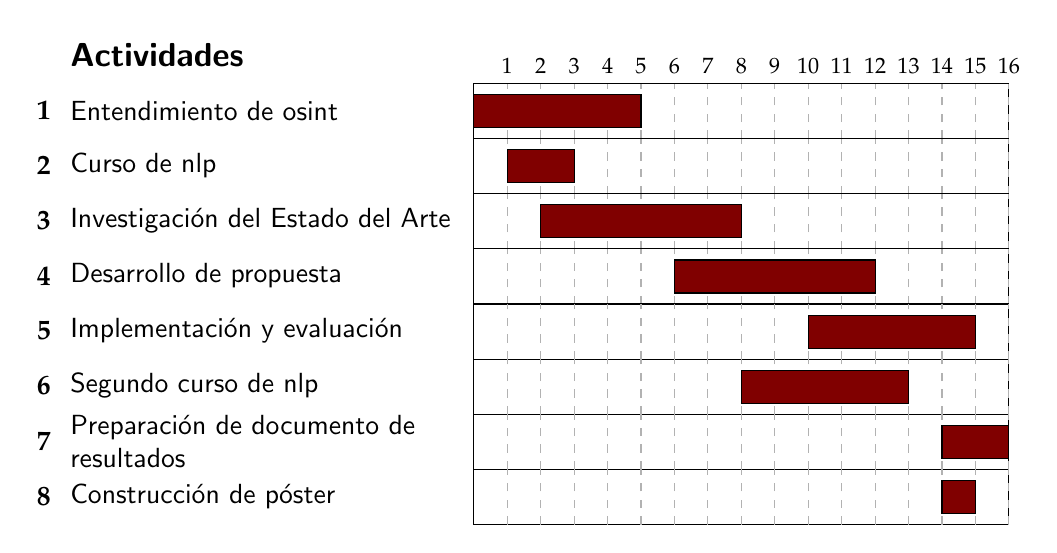
\begin{tikzpicture}
  \GanttHeader{\textwidth}{2ex}{5cm}{16}
  
  \Task{1}{Entendimiento de \gls{osint}}{0}{5}
  \Task{2}{Curso de \gls{nlp}}{1}{2}
  \Task{3}{Investigación del Estado del Arte}{2}{6}
  \Task{4}{Desarrollo de propuesta}{6}{6}
  \Task{5}{Implementación y evaluación}{10}{5}
  \Task{6}{Segundo curso de \gls{nlp}}{8}{5}
  \Task{7}{Preparación de documento de resultados}{14}{2}
  \Task{8}{Construcción de póster}{14}{1}
\end{tikzpicture}
\caption{Diagrama Gantt de actividades por semana de trabajo}
\label{fig:gantt}
\end{figure}

\vspace{1cm}

\begin{table}[h!]
\begin{center}
\begin{tabular}{|>{\centering\arraybackslash}p{.025\textwidth}|p{.975\textwidth}|} \hline
  & \textbf{Detalle} \\ \hline
  {\bf 1} & Entendimiento de \gls{nlp} y proyecto \gls{osint} \\ \hline
  
  {\bf 2} & Realización de curso de \gls{nlp} de \gls{udemy} \\ \hline
  
  {\bf 3} & Investigación del Estado del Arte \\ \hline
  
  {\bf 4} & Desarrollo de la propuesta de investigación \\ \hline
  
  {\bf 5} & Desarrollo de la implementación y pruebas \\ \hline
  
  {\bf 6} & Realización de curso de \gls{nlp} de National Research University Higher School of Economics
            de \gls{coursera} \\ \hline
  
  {\bf 7} & Preparación final de documento de libro de proyectos y articulo de investigación \\ \hline
  
  {\bf 8} & Contracción de póster para presentación en la Vitrina Académica \\ \hline
\end{tabular}
\end{center}
\caption{Detalle de cronograma de actividades}
\label{table:schedule}
\end{table}
\chapter{Logros y productos del proyecto} % Main chapter title

\label{chap:achievements} % For referencing the chapter elsewhere, use \ref{Chapter1}

% 1. Nombre del proyecto
% 1. Integrantes
% 1. Director
% 2. Agenda
% 3. Objetivo general y específicos (para todo el proyecto: PGR1 y PGR2)
% 4. Justificación del proyecto
% 5. Resultados propuestos
% 5. Productos obtenidos a la fecha (explicación técnica de los resultados) (Seccion 3)
% 6. Marco teorico (x3)
% 7. Problemas y soluciones
% 7. Modelo 1 (x3)
% 7. Modelo 2 (x3)
% 8. Trabajo futuro y conclusiones

Entre los logros y productos obtenidos durante la ejecución de este proyecto de grado se encuentran los siguientes: \todo{Revisar bien}

\begin{enumerate}
\item Entendimiento de las generalidades de \gls{datascience}:
  \begin{itemize}
  \item Tipos de \glsentrylong{machinel}
  \item Sistemas de detección de anomalías (\glsentrylong{anomalydetectionsys})
  \item Diferentes modalidades de \gls{clustering}
  \end{itemize}
\item Identificacion de modelos de \gls{nlp} aplicable para el perfilado de cibercriminales
\item Entendimiento de los modelos de clasificación y \gls{clustering}:
  \begin{itemize}
  \item Clasificador de Na\"ive Bayes
  \item Maquinas de soporte vectorial (\glsentrylong{svm})
  \item Mapas autoorganizados (\glsentrylong{som})
  \end{itemize}
\item Entendimiento de los modelos \gls{nlp}:
  \begin{itemize}
  \item Predicción de etiquetas con modelos de regresión lineal
  \item Reconocimiento de \gls{namedent}
  \item Uso de \emph{embeddings} generados con \gls{starspace} para los $k$ textos mas similares
  \end{itemize}
\item Implementación de modelos de \gls{nlp} para el perfilado de cibercriminales:
  \begin{itemize}
  \item Modelo de predicción de hashtags de Twitter con modelos lineales \todo{Por terminar}
  \item Modelo de reconocimiento de \gls{namedent} con redes \glsentrylong{lstm} \todo{Pendiente}
  \item Modelo de \gls{clustering} en redes \glsentrytext{som} con \emph{embeddings} de \gls{starspace} \todo{Por mirar}
  \end{itemize}
\end{enumerate}

\chapter{Marco teórico} % Main chapter title

\label{ch:MarcoTeorico} % For referencing the chapter elsewhere, use \ref{Chapter1} 

%----------------------------------------------------------------------------------------


La Web contiene una gran cantidad de opiniones respecto a productos, políticos, y mucho mas, expresado en forma de noticias, sitios de opinión, reseñas en tiendas online, redes sociales. Como resultado, el problema de ``Minería de opinión'' ha obtenido una atención creciente en las ultimas dos décadas y es un factor decisivo para las nuevas organizaciones (como es mencionado en \cite{Popescu2007}). De esto mismo partimos que el análisis de textos para extraer el significado y demás componentes extraíbles del texto componen un factor que debe considerarse al momento de realizar decisiones, de manera que los avances hechos hasta ahora tienen como meta una aplicación practica de lo que se conoce como \glsentrylong{nlp}.

Luego de los ataques terroristas del 11 de Septiembre de 2001 en Estados Unidos, se realizaron fuertes criticas respecto a la inteligencia, donde el director del FBI~\emph{Robert~S.~Mueller} indico que el principal problema que la agencia tuvo fue que se enfocaba demasiado en lidiar con el crimen luego de que fue cometido y ponía muy poco énfasis en prevenirlo (adaptado de \cite{mena2003investigative}). Es por esto que el uso de \gls{nlp} para temas de seguridad como también de metodologías de \glsentrylong{machinel} y \glsentrylong{deepl} han sido ampliamente utilizadas en ámbito de seguridad luego de estos eventos.

Para obtener una mejor inteligencia se necesito de mejores tecnologías a las que se tenían entonces (véase \cite[p\'ag 2]{mena2003investigative}):
\begin{itemize}
\item Integración de datos (\'o \gls{dataintegration} en ingl\'es)
\item Análisis de vínculos (\'o \gls{linkanalisys} en ingl\'es)
\item Agentes de software (\'o \gls{softwareagents} en ingl\'es)
\item Minería de texto (\'o \gls{textmining} en ingl\'es)
\item Redes neuronales (\'o \gls{neuralnetwork} en ingl\'es)
\item Algoritmos de \glsentrylong{machinel} (\'o \gls{mlalgorithms} en ingl\'es)
\end{itemize}

% ================================================================

\section{Análisis de vínculos (\glsentrylong{linkanalisys})}
Es la visualización de asociaciones entre entidades y eventos, por lo general involucran una visualización por medio de una gráfica o un mapa que muestre las relaciones entre sospechosos y ubicaciones, sea por medio físico o por comunicaciones en la red.

% ================================================================

\section{Agentes de software (\glsentrylong{softwareagents})}
Es el software que realiza tareas asignadas por el usuario de manera autónoma, donde sus habilidades básicas son:
\begin{itemize}
\item \textbf{Realización de tareas:} Hacen obtención de información, filtrado, monitoreo y reporte.
\item \textbf{Conocimiento:} Pueden usar reglas programadas, o pueden aprender reglas nuevas (véase \ref{sec:KBS}).
\item \textbf{Habilidades de comunicación:} Reportar a humanos e interactuar con otros agentes.
\end{itemize}

% ================================================================

\section{Aprendizaje de maquina (\glsentrylong{machinel})} \label{sec:ML}
De acuerdo con \cite{murphymachinel}, se define como un conjunto de métodos que pueden detectar patrones automáticamente en datos, y luego usar los patrones descubiertos para predecir los datos futuros, o realizar otra clase de toma de decisiones con un grado de incertidumbre, por tal motivo es necesario el uso de teoría de probabilidad, que puede ser aplicada a cualquier tipo de problema que involucra incertidumbre.

\subsection{Tipos de \glsentrylong{machinel}}
\gls{machinel} esta principalmente dividida en dos tipos. El método predictivo o bien \textbf{aprendizaje supervisado} (\gls{supervisedl}), donde el objetivo es aprender un mapeo de las entradas $\mathbf{x}$ a las salidas $y$, dado un conjunto de pares de etiquetas de entrada--salida $D = \{(\mathbf{x}_i, y_i)\}_{i=1}^{N}$. $D$ se le llama el conjunto de entrenamiento y $N$ es el numero de muestras de entrenamiento.

En la forma mas sencilla, cada entrada de entrenamiento $\mathbf{x}_i$ es un vector $D$--dimensional de números, a estos se le llaman \emph{características} o \emph{atributos}.

De manera similar la forma de la salida puede ser en principio cualquier cosa, pero la mayoría de métodos asumen que $y_i$ es una variable \emph{categórica} o \emph{nominal} de algún conjunto finito, $y_i \in \{1,\ldots,C\}$, o que $y_i$ es un escalar real, $y_i \in \mathbb{R}$. Cuando la variable $y_i$ es categórica, al problema se le reconoce como \textbf{clasificación} o \textbf{reconocimiento de patrones}, y cuando es un valor real se le conoce como un problema de \textbf{regresión}.

El segundo tipo principal de \gls{machinel} es el descriptivo o \textbf{aprendizaje no--supervisado} (\gls{unsupervisedl}), en este solo están disponibles los datos de entrada $D = \{\mathbf{x}_i\}_{i=1}^{N}$, y la meta es encontrar ``patrones interesantes'' en los datos. Este es un problema mucho menos definido, debido a que no se conocen los tipos de patrones que se quieren encontrar, y no hay una métrica obvia de error (no como aprendizaje supervisado en la que se puede comparar nuestra predicción de $y$ para un $\mathbf{x}$ con el valor observado).

Un tercer tipo de aprendizaje de maquina es conocido como \textbf{\gls{reinforcedl}}, el cual es un tipo menos usado. Este es útil cuando se quiere aprender como actuar o comportarse cuando se recibe una recompensa ocasional o una señal de castigo.

\subsection{Sistemas de Detección de Anomalías (\glsentrylong{anomalydetectionsys})}
Pendiente


% ================================================================
\section{Mineria de datos (\glsentrylong{datamining})} \label{sec:datamining}
Según \cite{tan2005introduction}, la minería de datos se define como el proceso de descubrir información útil en repositorios grandes de datos. Las técnicas de minería de datos son desplegadas para limpiar grandes bases de datos para encontrar patrones nuevos y útiles que de lo contrario podrían permanecer desconocidos. También ofrecen capacidades para predecir la salida de observaciones futuras, tales como predecir si un cliente nuevo gastara mas de \$100 en una tienda.

No todas las tareas de descubrimiento de información son considerados como \gls{datamining}. Por ejemplo, realizar una consulta de campos individuales usando un sistema de base de datos o encontrar una pagina web por medio de una búsqueda en Internet son tareas relacionadas con \emph{adquisición de información}.

\subsection{Mineria de texto (\glsentrylong{textmining})} \label{subsec:NLP}
Es un subcampo de Inteligencia Artificial conocida como \glsentrylong{nlp}, en donde las herramientas de minería de datos pueden capturar rasgos críticos del contenido de un documento basado en el análisis de sus características lingüísticas.

La mayoría de los crímenes son electrónicos por naturaleza, por lo que se dejan rastros textuales que investigadores pueden seguir y analizar. Estas se enfocan en el descubrimiento de relaciones en texto no--estructurado y pueden ser aplicados al problema de \emph{búsqueda} y \emph{localización de palabras clave}.

\subsection{Clasificación} \label{subsec:clasification}
Clasificación es la tarea de asignarle una de varias categorías predefinidas a objetos, y es una tarea que tiene una variedad extensa de aplicaciones. Ejemplos de esto se encuentran la detección de correos no deseados en mensajes de e--mails basándose del encabezado o el cuerpo del mensaje, categorización de células benignas de malignas basándose en los resultados de escaneados MRI o incluso la clasificación de galaxias basado en su forma.

Definido formalmente, clasificación es la tarea de aprender una función objetivo $f$ que mapea cada conjunto de atributos $x$ a una clase predefinida de etiquetas $y$.

La función objetivo también se define informalmente como un \emph{modelo de clasificación}.

\subsubsection{Metodologías de clasificación} \label{subsubsec:classmethods}
Existen muchos métodos para la clasificación de datos no--estructurados, entre los descritos aquí están:
\begin{itemize}
\item Clasificador basado en reglas (véase \ref{sec:KBS})
\item Redes neuronales artificiales (véase \ref{sec:ANN})
\item Maquinas de soporte vectorial (véase \ref{sec:SVM})
\item Clasificador de Na\"{\i}ve Bayes (véase \ref{subsec:naivebayes})
\end{itemize}

\subsection{Clustering} \label{subsec:clustering}
El análisis de clusters agrupa objetos de datos basándose únicamente en la información encontrada en los datos que describen los objetos y sus relaciones. El objetivo es que objetos dentro de un grupo sean similares (o relacionados) el uno al otro, y que sean diferentes (o sin relación) a objetos en otros grupos. Entre mayor sea la similitud dentro de un grupo y entre mayor sea la diferencia entre grupos, sera mejor o mas distintivo el clustering.

Los métodos de clustering se hacen referencia comúnmente en \gls{machinel} como métodos no--supervisados, los cuales se describen en \ref{sec:ML}. Un método de estos se describe en \ref{subsec:SOM} conocidos como mapas autoorganizados.

% ================================================================

\section{Sistemas Basados en Conocimiento (\glsentrylong{kbs})} \label{sec:KBS}
Según \cite{sajja2010knowledge}, los \gls{kbs} son uno de los mayores miembros de la familia de \gls{ai}. El \gls{kbs} consiste de una \gls{knowledgebase} y un programa de búsqueda llamado \gls{inferenceengine} representado en la figura \ref{fig:kbs-arch}. La \gls{knowledgebase} puede ser usado como un repositorio de conocimiento de varias formas.

Existen 5 tipos de \gls{kbs}, donde uno de ellos es conocido como \gls{expertsystems}, usados como \gls{rulebasedsys}, donde su \gls{knowledgebase} esta dado como reglas y el \gls{inferenceengine} esta dado por algo llamado \gls{workingmemory}, que representa los hechos que se conocen inicialmente del sistema junto con los hechos que se van dando como inferencia de las reglas.

\begin{figure}[H]
\centering
\includegraphics[scale=0.4]{Figures/kbs-architecture.png}
\decoRule
\caption[Arquitectura \glsentrytext{kbs}]{Arquitectura \glsentrytext{kbs}. Tomado de \cite{sajja2010knowledge}}
\label{fig:kbs-arch}
\end{figure}

Estas reglas pueden resumirse como una colección de condicionales de la forma \textbf{IF/ELSE} que se componen de un \emph{antecedente} y un \emph{consecuente}.

Existen dos tipos de \gls{rulebasedsys}, definidos como \gls{deductivesys} y \gls{reactivesys}, donde el \gls{deductivesys} tiene como objetivo realizar una conclusión en base a los hechos iniciales en la \gls{workingmemory}, por el otro lado se tienen los \gls{reactivesys}, los cuales de igual manera a los \gls{deductivesys}, toman los hechos de la \gls{workingmemory} y realizan sea una acción interactiva con su entorno o bien una modificación de los hechos que se encuentran en la \gls{workingmemory} tal como la adición o eliminación de hechos. Tómese el ejemplo de la ecuación \ref{eq:rbs-example} tomada de \cite{Mendel}, donde \emph{x} es la temperatura y \emph{AC} es aire acondicionado.

\begin{equation} \label{eq:rbs-example}
  \left\{ \begin{array}{ll}
            \text{IF x es moderado,} & \text{THEN y = ajustar AC a bajo} \\
            \text{IF x es alto,}     & \text{THEN y = ajustar AC a moderado a alto} \\
            \text{IF x es muy alto,} & \text{THEN y = ajustar AC a alto} 
          \end{array} \right.
\end{equation}

\subsection{Fuzzy Knowledge Based Systems}
Pendiente


% ================================================================

\section{Redes Neuronales Artificiales (\glsentrylong{neuralnetwork})} \label{sec:ANN}
El estudio de redes neuronales artificiales fue inspirado por los intentos de simular los sistemas biológicos de neuronas. El cerebro humano se compone principalmente de células nerviosas llamadas \emph{neuronas}, enlazadas con otras neuronas por medio de hebras de fibra conocidas como \emph{axones}. Los axones son usados para transmitir impulsos nerviosos de una neurona a otra cada vez que las neuronas son estimuladas. Una neurona esta conectada a axones de otras neuronas por medio de \emph{dendritas}, las cuales son extensiones desde el cuerpo de la neurona. El punto de contacto entre una dendrita y un axón se conoce como \emph{sinapsis}. Los neurólogos han descubierto que el cerebro humano aprende por medio de cambiar la fuerza de la conexión sináptica entre las neuronas a través de estimulación repetitiva por el mismo impulso.

De manera análoga a la estructura del cerebro humano, una \gls{neuralnetwork} se compone de una estructura interconectada de nodos y vínculos directos.

\subsection{Mapa autoorganizado (\glsentrylong{som})} \label{subsec:SOM}
El objetivo principal de los \gls{som} es de transformar una patrón de entrada $m$--dimensional en un mapa discreto uni-- o bi--dimensional, donde sus principales características es que es un algoritmo que se basa en \gls{unsupervisedl}, es \gls{feedforward}, tiene una sola capa de neuronas donde su propósito es realizar \gls{clustering} y una reducción de dimensionalidad sobre los datos de una forma topologicamente ordenada.

Los \gls{som} tienen tres características distintivas:
\begin{itemize}
\item {\bf Competencia:} por cada patrón de entrada, las neuronas en la red competirán entre ellas para determinar un ganador.
\item {\bf Cooperación:} la neurona ganadora determina la ubicación espacial (vecinos) alrededor de donde otras vecinas también se verán estimuladas.
\item {\bf Adaptación:} la neurona ganadora como también sus vecinas tendrán sus pesos asociados actualizados, y se tiene que los vecinos entre mas cerca estén del ganador, mayor es el grado de adaptación.
\end{itemize}

El algoritmo de aprendizaje de \gls{som} parte de primero inicializar los pesos de las $o$ neuronas con pesos aleatorios pequeños de una distribución de probabilidad aleatoria o uniforme, donde cada vector de entrada se define como $x = [x_1, \ldots, x_m]^{T} \in \mathbb{R}^{m}$ y la entrada general de $N$ patrones como $\mathbf{X}^{m \times N}$, el vector de pesos de la neurona $i$ es $\mathbf{w}_i = [w_{i1}, \ldots, w_{im}] \in \mathbb{R}^{1 \times m}$, con la matriz de pesos $\mathbf{W}^{o \times m}$.

Para alcanzar el objetivo de \emph{competencia}, se realiza por cada patrón de entrada $x_i$ una comparación con cada uno de los pesos de las $o$ neuronas y se establece la de menor distancia respecto $x_i$ (típicamente la distancia Euclidiana), dejando un ganador $winner$, tal como en la ecuación \ref{eq:som-competition}.
\begin{equation} \label{eq:som-competition}
  winner = \text{argmin}_j \norm{x_i - w_j} ; j = 1, \ldots,o
\end{equation}

Luego de establecer la neurona ganadora, se realiza el paso para alcanzar la \emph{cooperación}, que consiste en que por medio de una función kernel $h$ (típicamente una una distribución gaussiana), que permite establecer un área de afectación de las otras neuronas según su ubicación física en el mapa, definidos como $r_{winner}$ y $r_j$ que son la ubicación de la neurona ganadora y la neurona vecina $j$, en el cual el grado de afectación de la neurona vecina depende de la distancia de la que esta de la neurona ganadora, definido en la ecuación \ref{eq:som-cooperation}.
\begin{equation} \label{eq:som-cooperation}
  h_{j, winner}(t) = \text{exp}\Bigg(\frac{- \norm{r_j - r_{winner}}^2}{ 2 \sigma(t)^2}\Bigg)
\end{equation}

Parte importante del proceso de convergencia del \gls{som} es que a medida que avanzan las iteraciones $t$ del algoritmo el área de afectación se va reduciendo como parte del proceso de adaptación, por lo que definimos $\sigma(t) = \sigma_0 \text{exp}(-t / \tau_1)$, donde $\tau_1$ es una constante heurística y $\sigma_0$ la dimensión del mapa \gls{som}.

Finalmente para alcanzar la \emph{adaptación} se realiza una actualización de los pesos de la matriz $\mathbf{W}$ en base a la influencia de área $\sigma(t)$ y de una tasa de aprendizaje $\alpha(t) = \alpha_0 \text{exp}(-t/ \tau_2)$, donde $\tau_2$ es otra constante heurística y $\alpha_0$ es una constante de aprendizaje inicial, que debe ser $0 \le \alpha_0 \le 1$, la actualización se describe por la ecuación \ref{eq:som-adaptation} y el proceso puede ser visto gráficamente en la figura \ref{fig:som-adap-proc}, tanto de forma uni-- como bi--dimensional.
\begin{equation} \label{eq:som-adaptation}
  w_j(t+1) = w_j(t) + \alpha(t) h_{j, winner}(t)\Big[x_i-w_j(t)\Big]
\end{equation}

\begin{figure}[H]
\centering
\includegraphics[scale=0.2]{Figures/som-adaptive-proc.png}
\decoRule
\caption[Proceso de adaptación de \glsentrytext{som}]{Proceso de adaptación de \glsentrytext{som}, (a) uni--dimensional, (b) bi--dimensional. Tomado de \cite{de2006fundamentals}}
\label{fig:som-adap-proc}
\end{figure}

Luego de que el algoritmo de aprendizaje termina de realizar las iteraciones, la salida de este es la matriz de pesos $\mathbf{W}$, en la figura \ref{fig:som-impl-example} se puede apreciar una aproximación del algoritmo con un mapa uni--dimensional tratando de aproximar una función sinusoidal con ruido adicionado en un gráfico 2D.

\begin{figure}[H]
\centering
\includegraphics[scale=0.5]{Figures/som-implementation-example.png}
\decoRule
\caption[Ejemplo de salida de \glsentrytext{som}]{Ejemplo de salida de \glsentrytext{som}. Implementación propia.}
\label{fig:som-impl-example}
\end{figure}

\begin{figure}[H]
\centering
\includegraphics[scale=0.3]{Figures/som-example.png}
\decoRule
\caption[Ejemplo de uso de \glsentrytext{som} en aplicaciones de perfilado]{Ejemplo de uso de \glsentrytext{som} en aplicaciones de perfilado. Tomado de \cite{mena2003investigative}}
\label{fig:som-example}
\end{figure}

% ================================================================

\section{Maquina de soporte vectorial (\glsentrylong{svm})} \label{sec:SVM}
gls{svm} es una técnica de clasificación que tiene sus raíces en la teoría de aprendizaje estadístico que ha mostrado resultados empíricos prometedores en muchas aplicaciones practicas, desde reconocimiento de dígitos escritos a mano a categorización de texto. \gls{svm} también funciona muy bien con datos de alta dimensionalidad. Otro aspecto destacable de esta aproximación es que representa la frontera de decisión usando un subconjunto de las muestras de entrenamiento, conocidos como los \emph{support vectors}.

\subsection{Maximum Margin Hyperplanes}
Se puede entender a los \gls{mmh} como hiper-planos que ayudan a separar datos en un hiper-espacio y que poseen un margen de decisión entre los datos, como ejemplo tómese la figura \ref{fig:svm-hyperplanes}, donde el hiper-plano $B_1$ tiene un margen de decisión mas grande que el hiper-plano $B_2$.

\begin{figure}[H]
\centering
\includegraphics[scale=0.3]{Figures/svm-hyperplanes.png}
\decoRule
\caption[\glsentryname{mmh}]{\glsentryname{mmh}. Tomado de \cite{tan2005introduction}}
\label{fig:svm-hyperplanes}
\end{figure}

Finalmente, el objetivo final de los \gls{svm} es la búsqueda de un hiper-plano con el mayor margen de decisión. Existen dos tipos de \gls{svm}, el lineal y el no--lineal. El lineal realiza la separación de los datos con su hiper-plano a partir de los datos de entrada en su espacio vectorial original, mientras que el no--lineal consta de realizar una transformación de los espacios de los datos de entrada a uno en que sea linealmente separable (véase como ejemplo la figura \ref{fig:svm-nonlinear-transforms}), sin embargo al realizar la transformación, el algoritmo de \gls{svm} se ve afectado por la dimensionalidad de la entrada, por lo que existe lo que se conoce como la función \emph{kernel} para remediarlo.

\begin{figure}[H]
\centering
\includegraphics[scale=0.25]{Figures/svm-nonlinear-transform.png}
\decoRule
\caption[Transformación de espacios en \glsentrylong{svm}]{Transformación de espacios en \glsentrylong{svm}. Tomado de \cite{tan2005introduction}}
\label{fig:svm-nonlinear-transforms}
\end{figure}

\subsection{Función Kernel}
La función polinomial de similaridad, $K$, la cual es calculada en el espacio original de los datos de entrada, se le conoce como la \textbf{función Kernel}. En principio se asegura que la función kernel puede ser expresada siempre como el producto punto entre dos vectores de entrada en algún espacio de alta dimensionalidad, la función de kernel también tiene la particularidad de que el computo de los productos punto con la función toman considerablemente menos tiempo que realizar la transformación de espacios, dejando de lado la transformación, acelerando la tarea de clasificación.

% ================================================================

\section{Clasificadores Bayesianos} \label{sec:bayes}
En muchas aplicaciones de relaciones entre el conjunto de atributos y la etiqueta es no--determinante. Es decir, la etiqueta de clase de un dato de un conjunto de prueba no puede ser determinado con certeza a pesar de ser un atributo idéntico a los atributos de entrenamiento. Esto puede ser producto de que los datos poseen ruido o la presencia de ciertos factores que afectan la clasificación pero no son incluidos en el análisis. Para esto es crucial el teorema de Bayes, el cual es un principio estadístico que combina el conocimiento previo de las clases con la nueva evidencia que se obtiene de los datos.

\subsection{Teorema de Bayes} \label{subsec:bayestheo}
El teorema de Bayes dice que para un par de variables aleatorias $X$ y $Y$ y que $P(X=x | Y=y)$ la probabilidad de que la variable $X$ tome el valor $x$ dado que el valor de la variable $Y$ es $y$. Se tiene entonces la ecuación \ref{eq:bayestheo}.
\begin{equation} \label{eq:bayestheo}
  P(Y | X) = \frac{P(X | Y) P(Y)}{P(X)}
\end{equation}

\subsubsection{Usando el teorema de Bayes para clasificación}
Para denotar el problema de clasificación desde una perspectiva estadística se define a $X$ como el conjunto de atributos y $Y$ como el conjunto de etiquetas de clase. Si la etiqueta de clase tiene una relación no--determinante con los atributos, entonces se pueden tomar a $X$ y a $Y$ como variables aleatorias y capturar su relación probabilística con $P(Y|X)$, conocida como la probabilidad posterior para $Y$, dada su probabilidad previa $P(Y)$.

Durante la fase de entrenamiento, es necesario aprender las probabilidades posteriores $P(Y|X)$ para cualquier combinación de $X$ y $Y$ basándose en la información recolectada de los datos de entrenamiento.

Dado que lo que se quiere realizar es una clasificación que represente la probabilidad de que dado un valor de $X=x$ este relacionado con que $Y=y$, se puede reconocer primero que $X$ se mantiene constante para lo que son los datos de entrenamiento, y que lo desconocido sea la clasificación $Y=y$ con probabilidad $P(Y|X)$, al conocer esta probabilidad, un valor de prueba $X'$ puede ser clasificado por medio de encontrar la clase $Y'$ que maximice la probabilidad posterior $P(Y'|X')$.


\subsection{Clasificador Na\"{\i}ve Bayes} \label{subsec:naivebayes}
Un clasificador de Na\"{\i}ve Bayes estima la probabilidad condicional de las clases por medio de suponer que los atributos son condicionalmente independientes, dado la etiqueta de clasificación $y$. La suposición de independencia condicional se puede dar por la ecuación \ref{eq:bayes-conditional-independence}.

\begin{equation} \label{eq:bayes-conditional-independence}
  P(X|Y=y) = \prod_{i=1}^{d} P(X_i|Y=y)
\end{equation}

Donde cada conjunto de atributos $X=\{ X_1, \ldots, X_d \}$ que consiste de $d$ atributos.
\subsubsection{Como funciona el clasificador Na\"{\i}ve Bayes}
Con la suposición de independencia condicional, en vez de computar la probabilidad condicional de clases para cada combinación de $X$, solo se debe realizar para establecer la probabilidad condicional de cada $X_i$, dado $Y$.

Para clasificar un dato de prueba, el clasificador computa la probabilidad posterior para cada clase $Y$ como se muestra en la ecuación \ref{eq:bayes-classifier}.

\begin{equation} \label{eq:bayes-classifier}
  P(Y|X) = \frac{P(Y) \prod_{i=1}^{d}P(X_i|Y)}{P(X)}
\end{equation}


\chapter{Estado del arte} % Main chapter title

\label{chStateOfTheArt} % For referencing the chapter elsewhere, use \ref{Chapter1} 

%----------------------------------------------------------------------------------------


La Web contiene una gran cantidad de opiniones respecto a productos, políticos, y mucho mas, expresado en forma de noticias, sitios de opinión, reseñas en tiendas online, redes sociales. Como resultado, el problema de ``Minería de opinión'' ha obtenido una atención creciente en las ultimas dos décadas y es un factor decisivo para las nuevas organizaciones. De esto mismo partimos que el análisis de textos para extraer el significado y demás componentes extraíbles del texto componen un factor que debe considerarse al momento de realizar decisiones, de manera que los avances hechos hasta ahora tienen como meta una aplicación practica de lo que se conoce como \glsentrylong{nlp}.

Luego de los ataques terroristas del 11 de Septiembre de 2001 en Estados Unidos, se realizaron fuertes criticas respecto a la inteligencia, donde el director del FBI~\emph{Robert~S.~Mueller} indico que el principal problema que la agencia tuvo fue que se enfocaba demasiado en lidiar con el crimen luego de que fue cometido y ponía muy poco énfasis en prevenirlo. Es por esto que el uso de \gls{nlp} para temas de seguridad como también de metodologías de \glsentrylong{machinel} y \glsentrylong{deepl} han sido ampliamente utilizadas en ámbito de seguridad luego de estos eventos.

Para obtener una mejor inteligencia se necesito de mejores tecnologías a las que se tenían entonces (véase \cite[p\'ag 2]{mena2003investigative}):
\begin{itemize}
\item Integración de datos (\'o \gls{dataintegration} en ingl\'es)
\item Análisis de vínculos (\'o \gls{linkanalisys} en ingl\'es)
\item Agentes de software (\'o \gls{softwareagents} en ingl\'es)
\item Minería de texto (\'o \gls{textmining} en ingl\'es)
\item Redes neuronales (\'o \gls{neuralnetworks} en ingl\'es)
\item Algoritmos de \glsentrylong{machinel} (\'o \gls{mlalgorithms} en ingl\'es)
\end{itemize}

% ================================================================

\section{Análisis de vínculos (\glsentrylong{linkanalisys})}
Es la visualización de asociaciones entre entidades y eventos, por lo general involucran una visualización por medio de una gráfica o un mapa que muestre las relaciones entre sospechosos y ubicaciones, sea por medio físico o por comunicaciones en la red.

% ================================================================

\section{Agentes de software (\glsentrylong{softwareagents})}
Es el software que realiza tareas asignadas por el usuario de manera autónoma, donde sus habilidades básicas son:
\begin{itemize}
\item \textbf{Realización de tareas:} Hacen obtención de información, filtrado, monitoreo y reporte.
\item \textbf{Conocimiento:} Pueden usar reglas programadas, o pueden aprender reglas nuevas (véase \ref{secKBS}).
\item \textbf{Habilidades de comunicación:} Reportar a humanos e interactuar con otros agentes.
\end{itemize}

% ================================================================

\section{Sistemas Basados en Conocimiento (\glsentrylong{kbs})} \label{secKBS}
Según \cite{sajja2010knowledge}, los \gls{kbs} son uno de los mayores miembros de la familia de \gls{ai}.

\begin{figure}[th]
\centering
\includegraphics[scale=0.4]{Figures/kbs-architecture.png}
\decoRule
\caption[Arquitectura \gls{kbs}]{Arquitectura \gls{kbs}. Tomado de \cite{sajja2010knowledge}}
\label{fig:KBSArch}
\end{figure}

\subsection{Fuzzy Knowledge Based Systems}
Pendiente

% ================================================================

\section{Mineria de texto (\glsentrylong{textmining})} \label{secNLP}
Es un subcampo de Inteligencia Artificial conocida como \glsentrylong{nlp}, en donde las herramientas de minería de datos pueden capturar rasgos críticos del contenido de un documento basado en el análisis de sus características lingüísticas.

La mayoría de los crímenes son electrónicos por naturaleza, por lo que se dejan rastros textuales que investigadores pueden seguir y analizar.Estas se enfocan en el descubrimiento de relaciones en texto no--estructurado y pueden ser aplicados al problema de \emph{búsqueda} y \emph{localizar palabras clave}.

% ================================================================

\section{Redes Neuronales (\glsentrylong{neuralnetworks})} \label{secNN}
Pendiente

\subsection{Sistemas de Detección de Anomalías (\glsentrylong{anomalydetectionsys})}
Pendiente

\subsection{Mapa autoorganizado (\glsentrylong{som})}
Pendiente

% ================================================================

\section{Aprendizaje de maquina (\glsentrylong{machinel})} \label{secML}
Pendiente
% Chapter 3

\chapter{Propuesta de aplicación} % Main chapter title
% \chapter{Propuesta de aplicación de modelos \glsentrytext{nlp} para el desarrollo de labores de inteligencia en escenarios de ciberterrorismo} % Main chapter title

\label{chap:proposal} % For referencing the chapter elsewhere, use \ref{Chapter1} 

%----------------------------------------------------------------------------------------

\newcommand{\nmodels}{$n$ \todo{?`cuantos modelos?}}

La propuesta consta de a aplicación de modelos de \glsentrytext{nlp} para el desarrollo de labores de inteligencia en escenarios de ciberterrorismo por medio de \nmodels modelos, pensados para el análisis de texto en redes sociales como Twitter en aras de realizar un perfilado de ciber-criminales potenciales, esto por medio de \gls{nlp}, de donde se parte varias metodologías que hacen uso de tecnologías \mbox{Estado-del-Arte}.

\section{Entendimiento del negocio (Business understanding)}
\todo{Pendiente}

\section{Adquisición de datos (Data acquisition)}
\todo[inline]{Incluir proceso de recolección por el API de Twitter o usando los datasets que estan en Archive}

\section{Modelamiento (Modelling)}
Como parte de la propuesta se proponen \nmodels modelos para tratar diferentes aspectos en perfilado de donde se representan los diferentes modelos en la \figureref{fig:proposal-arch}.

\begin{figure}[H]
  \centering
  % \missingfigure{Hacer la arquitectura en yEd}
  \includegraphics[width=\textwidth]{Figures/general-architecture.pdf}
\decoRule
\caption[Arquitectura de propuesta]{Arquitectura de propuesta.}
\label{fig:proposal-arch}
\end{figure}

\subsection{Modelo 1: Predicción de etiquetas de Twitter con modelos lineales} \label{sec:twitter-prediction}
En Twitter, las publicaciones que se realizan tienen la posibilidad de incluir menciones de temas de tendencia por el conocido \emph{hashtag}, escrito como \texttt{\#Tema}, y tiene la gran utilidad de realizar una mención explicita del tema que se quiere tratar y donde además la tarea de encontrar textos directamente relacionados con un tema son fácilmente localizables.

Así mismo, en la literatura de \gls{nlp} es muy común el uso de diferentes representaciones de palabras o conjuntos de palabras. Una representación de palabras típicas es por medio de los \gls{bow}, donde se establece un diccionario de palabras de tamaño $N$, y donde cada palabra tiene un vector que lo representa. A cada palabra se le asigna un identificador único en ese diccionario, por lo que existiría una traducción de palabra a identificador y una secuencia de palabras para poder ser recuperado por medio del índice, como se muestra en la \equationref{eq:bow-repr1} y la \equationref{eq:bow-repr2}.
\begin{equation} \label{eq:bow-repr1}
  \text{word2idx} = \Big\{(\text{word}_i, i) : \forall i \in \{1, \ldots, N\} \Big\}
\end{equation}

\begin{equation} \label{eq:bow-repr2}
  \text{idx2word} = \Big[\text{word}_i\Big], \forall i \in \{1, \ldots, N\}
\end{equation}

Otra representación común en \gls{nlp} es la de \gls{tfidf}, que se divide en dos partes, expresadas en las \equationref{eq:tf-repr}, la \equationref{eq:idf-repr} y la composición de ambas en la \equationref{eq:tfidf-repr}, $D$ es el corpus de palabras. Este consiste en penalizar palabras que ocurren mucho en un documento pero no mucho en el corpus o bien de penalizar la palabras que se repiten poco en un documento pero se repiten mucho en el corpus, por lo que un punto medio entre ambos es recompensado.

\begin{equation} \label{eq:tf-repr}
  \text{tf}(t,d) = \text{Frecuencia del termino (o n--grama) } t \text{ en el documento } d
\end{equation}

Existen diferentes variaciones para realizar representar el conteo de términos \textbf{tf} de forma normalizada, como se representa en el \tableref{table:tf}.

\begin{table}[h!]
\centering
\begin{tabular}{|l|l|} \hline
  \textbf{Esquema}          & \textbf{Peso de tf} \\ \hline
  Binario                   & $0, 1$ \\ \hline
  Conteo directo            & $f_{t, d}$ \\ \hline
  Frecuencia de términos    & $f_{t, d} / \sum_{t' \in d}f_{t', d}$ \\ \hline
  Normalización logarítmica & $1 + \text{log}(f_{f, d})$ \\ \hline
\end{tabular}
\caption{Variaciones de \textbf{tf}}
\label{table:tf}
\end{table}

\begin{equation} \label{eq:idf-repr}
  \text{idf}(t, D) = \text{log}\Bigg( \frac{N}{|\{d \in D : t \in d\}|} \Bigg) ; N = |D|
\end{equation}

\begin{equation} \label{eq:tfidf-repr}
  \text{tf-idf}(t, d, D) = \text{tf}(t, d) \cdot \text{idf}(t, D)
\end{equation}

\subsubsection{Creación del Corpus de palabras}
Debido a que los textos que se encuentran en Twitter no tienen forma estructurada es necesario realizar un preprocesamiento de cada post recolectado para luego contar la frecuencia de cada palabra dentro del corpus y así establecer las primeras $N$ palabras mas usadas que van a componer el corpus de palabras.

Para realizar el preprocesamiento de cada texto se hacen los siguientes pasos:
\begin{enumerate}
\item Convertir todas las palabras a minúscula (e.g. \mbox{``LaTeX'' $\rightarrow$ ``latex''})
\item Reemplazar todos los caracteres especiales de texto a espacios en blanco (e.g. \mbox{``\texttt{@;,:\textbackslash n\textbackslash t\textbackslash r}'' $\rightarrow$ ``\textvisiblespace \textvisiblespace \textvisiblespace \textvisiblespace \textvisiblespace \textvisiblespace \textvisiblespace''})
\item Remover todos los símbolos extraños, es decir todo lo que no sean numeros, ni letras ni los simbolos que se encuentran normalmente en tweets (e.g. \mbox{``\texttt{\%()\*\&\$!\^}'' $\rightarrow$ ``''})
\item Remover todas las \emph{stopwords}, que son palabras que no añaden ningún valor semántico al texto \\ (e.g. \mbox{``las palabras son una forma de expresarnos'' $\rightarrow$ ``palabras forma expresarnos''})
\end{enumerate}

Luego se realiza un conteo de todas la palabras presentes dentro del corpus de donde se sacan las $N$ primeras palabras para incluirlas en el \gls{bow}.

Luego de esto se generan las etiquetas (\'o \emph{tags} en ingles) que se toman directamente de los textos de entrenamiento, de estos también se les realiza un conteo, que servirán para la predicción de las etiquetas según el contenido del texto.

\subsubsection{Conversión de textos a vectores}
Para realizar la conversión de textos a vectores y así poder representar un texto como un vector se procede a primera realizar una generación de identificadores para cada palabra de manera como se describió en el inicio de la \sectionref{sec:twitter-prediction}.

La manera en que se representa un texto en forma de vector $\vs$ es por medio de la sumatoria de los vectores que representan cada palabra como se representa en la \equationref{eq:bow-word-vector-sum}, recuérdese que $\ve^{(i)}$ es un vector con un $1$ en la posición $i$ y ceros en el resto del vector.

\begin{equation} \label{eq:bow-word-vector-sum}
  \vs = \mathlarger{\mathlarger{\sum}}_{(\text{word}, i) \in \text{word2idx}} \ve^{(i)}, \text{word} \in d
\end{equation}

\subsubsection{Generación del conjunto de entrenamiento, validación y pruebas}
Para la generación de los conjuntos se toman las sumatorias generadas de cada tweet en su forma de vector y se coloca en una matriz de $\mT^{m \times N}$, donde $m$ son el numero de muestras de Twitter y $N$ el tamaño del Corpus.

\subsubsection{Clasificador de regresión logística}
\todo[inline]{Pendiente}

\subsubsection{Multiclasificador de One VS Rest}
\todo[inline]{Pendiente: incluir arquitectura de solución en la \figureref{fig:model1-arch}}
\begin{figure}[H]
  \centering
  \missingfigure{Hacer la arquitectura en yEd}
  % \includegraphics[width=\textwidth]{Figures/general-architecture.pdf}
\decoRule
\caption[Arquitectura de Modelo 1]{Arquitectura de Modelo 1.}
\label{fig:model1-arch}
\end{figure}

%----------------------------------------------------------------------------------------

\subsection{Modelo 2: Reconocimiento de \glsentrylong{namedent} con redes \glsentrylong{lstm}}
\todo{Pendiente} Bla
\todo{incluir diagramas de pagina de Google}

\subsection{Modelo 3: Búsqueda de tweets relacionados con \emph{embeddings} de StarSpace}
\todo{Pendiente} Bla


\section{Despliegue (Deployment)}
\todo{Pendiente}
\lipsum{1}


%----------------------------------------------------------------------------------------
%	THESIS CONTENT - APPENDICES
%----------------------------------------------------------------------------------------

\appendix % Cue to tell LaTeX that the following "chapters" are Appendices

% Include the appendices of the thesis as separate files from the Appendices folder
% Uncomment the lines as you write the Appendices
% \include{Appendices/AppendixA}
%\include{Appendices/AppendixC}

% \glsaddall
% \printglossary[title={Abreviaturas},type=\acronymtype]
\setglossarystyle{altlistgroup}
\printglossary[type=main]

% \printindex

%----------------------------------------------------------------------------------------
%	BIBLIOGRAPHY
%----------------------------------------------------------------------------------------

\nocite{*}
\printbibliography[heading=bibintoc]

%----------------------------------------------------------------------------------------

\end{document}  
